\subsubsection{Mémoire distribuée}
Pour paralléliser un produit matrice vecteur creux en mémoire distribuée, il faut tout d'abord distribuer la matrice sur tous les processus.
%
Chaque processus devra s'occuper d'un ensemble de lignes de la matrice.
%
Cette répartition sera statique et les indices des lignes seront les mêmes pour la distribution des vecteurs (Fig.~\ref{fig:spmv_mpi}).
%
Nous pouvons voir que certains éléments du vecteur $x$ doivent être partagés.
%
Pour cela, l'algorithme démarrera par une phase de communication de ces éléments.
%
Puis chaque processus pourra effectuer la multiplication de ces lignes de matrice et stocker le résultat dans un vecteur $y$ local.
%   (-_-)   %
\begin{figure}
  \centering
  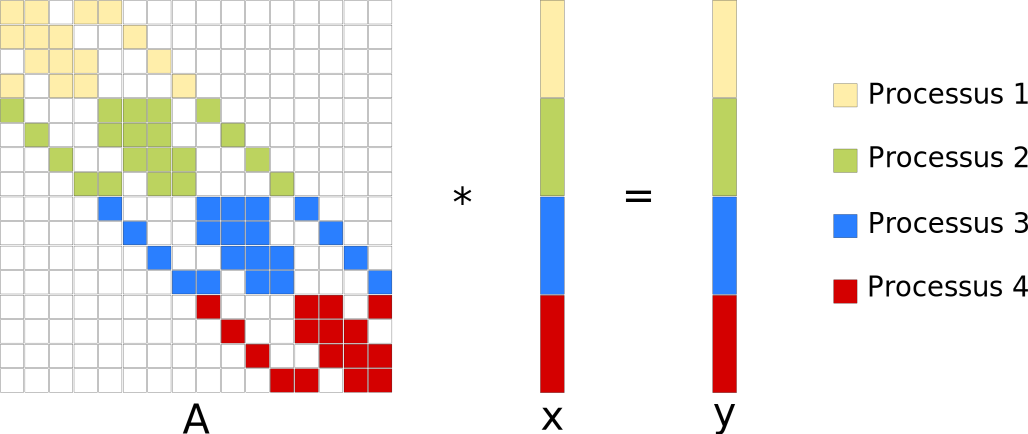
\includegraphics[width=\textwidth]{spmv_mpi}
  \caption{Distribution des données utilisées par le produit matrice vecteur creux.}
  \label{fig:spmv_mpi}
\end{figure}
Hormis la phase de communication au début de l'algorithme, le SpMV se parallélise très bien en mémoire distribuée.
%
Cette phase de communication peut être, dans certains cas, recouverte par du calcul.
%
Il suffit de multiplier en premier les lignes de la matrice qui ne dépendent pas des éléments distants.
%
Puis une fois les éléments reçus, il est possible de multiplier les lignes restantes.

La performance atteinte en mémoire distribuée correspond à la performance crête du SpMV.
%
En effet, de par sa nature distribuée, les pénalités mémoires NUMA sont minimales.
%
Chaque processus allouera la mémoire dont il a besoin sur son propre banc NUMA et si celui-ci n'est pas déplacé, tous ces accès mémoires seront optimaux.
%
Nous pouvons donc estimer cette performance sera la borne maximale à atteindre lorsque l'on travaillera en mémoire partagée.


Le roofline model prédit un algorithme limité en performance par la bande passante mémoire.
%
Or, cette bande passante mémoire est partagée entre les coeurs d'un même banc NUMA.
%
L'accélération obtenue sera donc limitée par la bande passante mémoire.
%
Sur la machine Rostand, la bande passante mémoire limite grandement cette accélération (Fig.~\ref{fig:res_spmv_mpi_rostand}).
%
Avec un cas à 8 variables primaires, nous obtenons une accélération maximale de 3,8.
%
La capacité de calcul mesuré avec 12 coeurs est de 4,96~GFlops, cela correspond à la prédiction du roofline model.

Sur Manumanu, nous avons beaucoup plus de bancs NUMA, ce qui signifie que nous aurons plus de bande passante mémoire à notre disposition.
%
Nous pouvons donc espérer avoir de meilleurs résultats que sur Rostand.
%
Il faut aussi prendre en compte une bande passante mémoire plus élevée sur les bancs NUMA de Manumanu que sur ceux de Rostand.
%
Nous avons choisi d'allouer les processus MPI en mode compact, c'est-à-dire qu'ils sont distribués de façon à utiliser un minimum de noeuds NUMA.
%
Nous pourrons ainsi voir les différents paliers tous les 8 coeurs qui correspondent à l'ajout de bande passante mémoire d'un nouveau processeur.
%
Ces paliers sont difficilement visibles sur la courbe des résultats (Fig.~\ref{fig:res_spmv_mpi_manu}).
%
Mais les valeurs numériques sont plus expressives, par exemple avec 1 variable primaire, l'accélération sur 7 et 8 coeurs est la même (4,72), l'utilisation d'un neuvième coeur la fait augmenter (5,34).
%
Sur 1 banc NUMA, nous avons une accélération de 6 avec 8 variables primaires.
%
Cette accélération monte à 110 avec l'utilisation des 20 bancs NUMA et des 160 coeurs.
%
Les performances par banc NUMA sont meilleures que sur Rostand.
%
Le passage à l'échelle entre 1 banc NUMA et 20 bancs NUMA est quasiment parfait.
